%%%%%%%%%%%%%%%%%%%%%%%%%%%%%%%%%%%%%%%%%
% Beamer Presentation
% LaTeX Template
% Version 1.0 (10/11/12)
%
% This template has been downloaded from:
% http://www.LaTeXTemplates.com
%
% License:
% CC BY-NC-SA 3.0 (http://creativecommons.org/licenses/by-nc-sa/3.0/)
%
%%%%%%%%%%%%%%%%%%%%%%%%%%%%%%%%%%%%%%%%%

%----------------------------------------------------------------------------------------
%	PACKAGES AND THEMES
%----------------------------------------------------------------------------------------

\documentclass{beamer}

\mode<presentation> {

% The Beamer class comes with a number of default slide themes
% which change the colors and layouts of slides. Below this is a list
% of all the themes, uncomment each in turn to see what they look like.

%\usetheme{default}
%\usetheme{AnnArbor}
%\usetheme{Antibes}
%\usetheme{Bergen}
%\usetheme{Berkeley}
\usetheme{Berlin}
%\usetheme{Boadilla}
%\usetheme{CambridgeUS}
%\usetheme{Copenhagen}
%\usetheme{Darmstadt}
%\usetheme{Dresden}
%\usetheme{Frankfurt}
%\usetheme{Goettingen}
%\usetheme{Hannover}
%\usetheme{Ilmenau}
%\usetheme{JuanLesPins}
%\usetheme{Luebeck}
%\usetheme{Madrid}
%\usetheme{Malmoe}
%\usetheme{Marburg}
%\usetheme{Montpellier}
%\usetheme{PaloAlto}
%\usetheme{Pittsburgh}
%\usetheme{Rochester}
%\usetheme{Singapore}
%\usetheme{Szeged}
%\usetheme{Warsaw}

% As well as themes, the Beamer class has a number of color themes
% for any slide theme. Uncomment each of these in turn to see how it
% changes the colors of your current slide theme.

%\usecolortheme{albatross}
%\usecolortheme{beaver}
%\usecolortheme{beetle}
%\usecolortheme{crane}
%\usecolortheme{dolphin}
%\usecolortheme{dove}
%\usecolortheme{fly}
%\usecolortheme{lily}
%\usecolortheme{orchid}
%\usecolortheme{rose}
%\usecolortheme{seagull}
%\usecolortheme{seahorse}
%\usecolortheme{whale}
%\usecolortheme{wolverine}

%\setbeamertemplate{footline} % To remove the footer line in all slides uncomment this line
\setbeamertemplate{footline}[page number] % To replace the footer line in all slides with a simple slide count uncomment this line

\setbeamertemplate{navigation symbols}{} % To remove the navigation symbols from the bottom of all slides uncomment this line
}

\usepackage{graphicx} % Allows including images
\usepackage{booktabs} % Allows the use of \toprule, \midrule and \bottomrule in tables
%\usepackage[brazilian]{babel}
\usepackage[utf8]{inputenc}
\usepackage{listings}
\usepackage{amsmath}
\usepackage{amsfonts}
\usepackage{pdfpages}
\usepackage{textpos}
\usepackage{caption}

\usepackage{subcaption} %Support for sub figures

% Para algoritmos
\usepackage{amsfonts}
\usepackage{algpseudocode}
\usepackage{algorithm}
\usepackage{algorithmicx}

\usepackage{appendixnumberbeamer}

\graphicspath{ {img/} }

%----------------------------------------------------------------------------------------
%	TITLE PAGE
%----------------------------------------------------------------------------------------

\title[Synchronizing Relations in Java]{Towards Synchronizing Relations Between Artifacts in the Java Technological Space} % The short title appears at the bottom of every slide, the full title is only on the title page

\author[William]{
\vskip 12pt
Author: William Bombardelli da Silva\\
Advisor: Dr.-Ing. Frank Trollmann} % Your name
\institute[TU Berlin] % Your institution as it will appear on the bottom of every slide, may be shorthand to save space
{
\vskip 12pt
Technische Universität Berlin \\ % Your institution for the title page
Fakultät IV Elektrotechnik und Informatik \\
Bachelorstudiengang Informatik \\
\medskip
\textit{wbombardellis@win.tu-berlin.de} % Your email address
}
\date{16.03.2016} % Date, can be changed to a custom date

\begin{document}

\begin{frame}
	\titlepage % Print the title page as the first slide
\end{frame}

\begin{frame}
	\frametitle{Organization} % Table of contents slide, comment this block out to remove it
	\tableofcontents % Throughout your presentation, if you choose to use \section{} and \subsection{} commands, these will automatically be printed on this slide as an overview of your presentation
\end{frame}

%----------------------------------------------------------------------------------------
%	PRESENTATION SLIDES
%----------------------------------------------------------------------------------------

%------------------------------------------------
\section{Introduction} % Sections can be created in order to organize your presentation into discrete blocks, all sections and subsections are automatically printed in the table of contents as an overview of the talk
%------------------------------------------------
%-------------------
% Subsection
%-------------------
\subsection{Background}
\begin{frame}
	\frametitle{Background}
	\tableofcontents[currentsection, currentsubsection] 
\end{frame}

\begin{frame}
	\frametitle{Models are used in Software Engineering}
	\begin{figure}[H]
		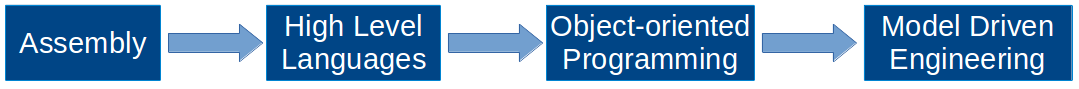
\includegraphics[width=\textwidth]{LanguagesHystoryDiagram}
	\end{figure}
	\pause
	\begin{itemize}
		\item New needs in industry thrill new methods and paradigms.
		\item \textbf{Model-driven Engineering (MDE):} Software processes are oriented to models.
		\item One software may have several different models.
	\end{itemize}
\end{frame}

\begin{frame}
	\frametitle{Models have to be kept consistent}
	\begin{figure}[H]
		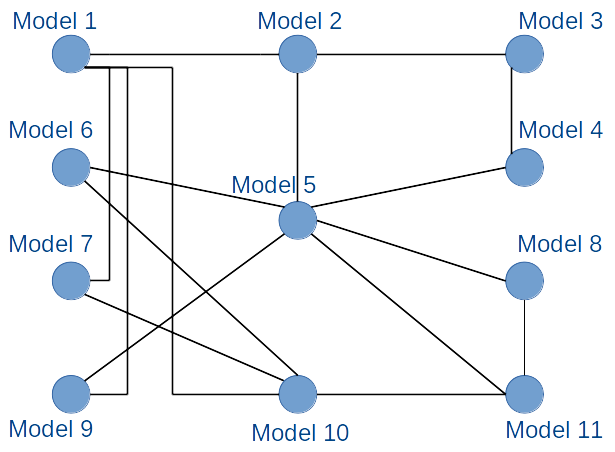
\includegraphics[scale=0.3]{network_models_generic}
	\end{figure}
	\pause
	\begin{itemize}
		\item Models are to be maintained consistent as they evolve.
		\item This means \textbf{models synchronization}.
	\end{itemize}
\end{frame}

\begin{frame}[t]
	\frametitle{Model Synchronization in the Network of Models}		\nocite{diskin2011model}
	\begin{itemize}
		\item For each edge of the network there is a synchronization task.
	\end{itemize}
	\only<2>{
		\begin{figure}
			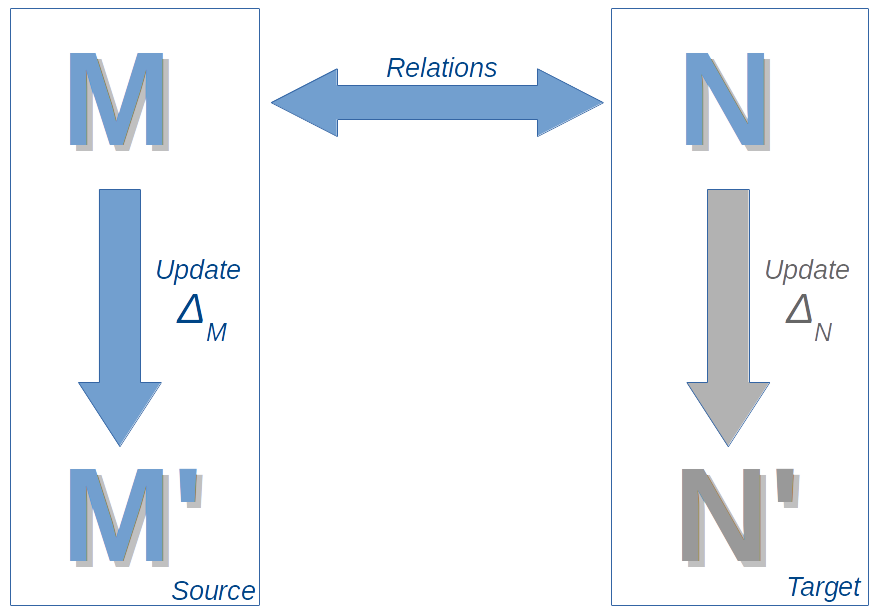
\includegraphics[width=.7\textwidth]{fooSynchronization}
		\end{figure}
	}
	\only<3>{
		\begin{figure}
			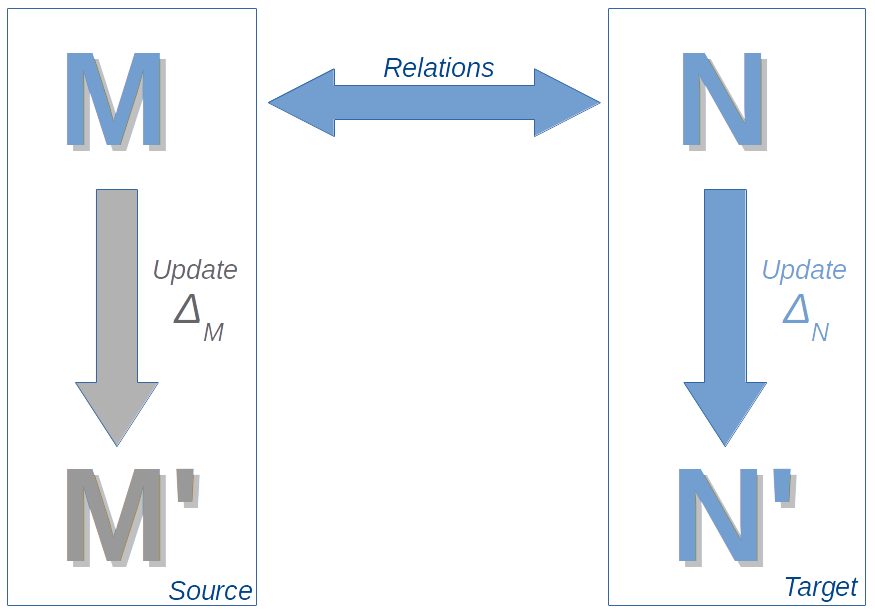
\includegraphics[width=.7\textwidth]{fooSynchronization_backward}
		\end{figure}
	}
\end{frame}

\begin{frame}[t]
	\frametitle{Relations are written between metamodels}
	\begin{figure}
		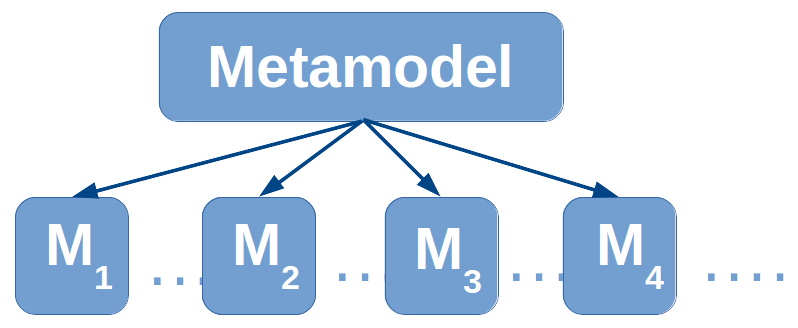
\includegraphics[scale=0.14]{metamodels_generic}
	\end{figure}
	\pause
	\vskip -10pt
	\begin{figure}
		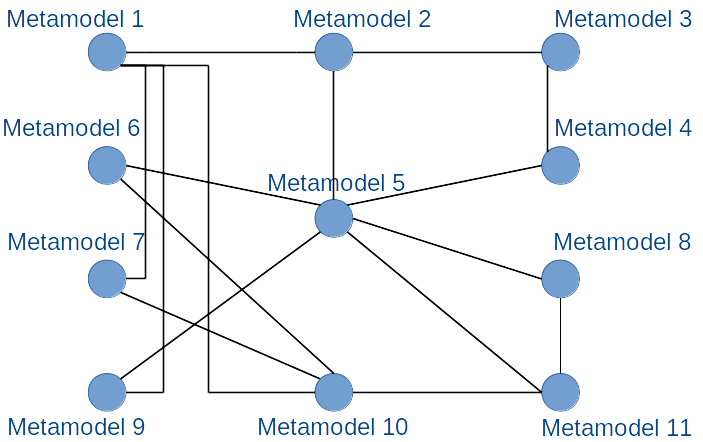
\includegraphics[scale=0.30]{network_metamodels_generic}
	\end{figure}
\end{frame}

%TODO: solltest du kurz auf die Einschränkungen der aktuelle State oft he Art eingehen, um für den Zuhörer zu motivieren warum dein Ansatz notwendig ist.

%-------------------
% Subsection
%-------------------
\subsection{Objective}
\begin{frame}
	\frametitle{Objective}
	\tableofcontents[currentsection, currentsubsection] 
\end{frame}

\begin{frame}[t]
	\frametitle{Three Steps}
	\begin{itemize}
		\item Focus on the Java technological space.
	\end{itemize}
	\pause
	\begin{figure}
		\vskip -5pt
		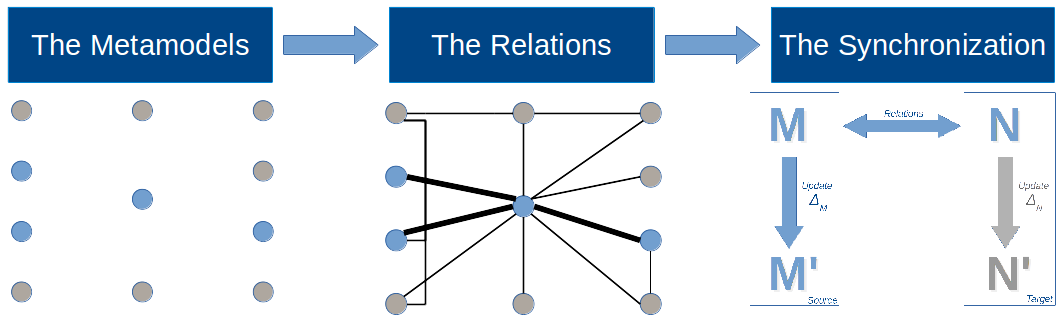
\includegraphics[scale=0.3]{objective}
	\end{figure}
\end{frame}

%------------------------------------------------
\section{Development} % Sections can be created in order to organize your presentation into discrete blocks, all sections and subsections are automatically printed in the table of contents as an overview of the talk
%------------------------------------------------
%-------------------
% Subsection
%-------------------
\subsection{The Metamodels}
\begin{frame}
	\frametitle{The Metamodels}
	\tableofcontents[currentsection, currentsubsection] 
\end{frame}

\begin{frame}
	\frametitle{Some Metamodels of the Java Technological Space}
	\begin{figure}
		\vskip -5pt
		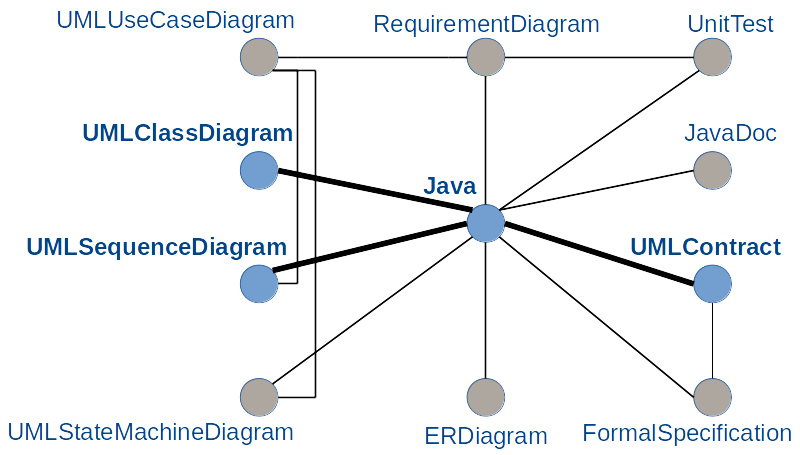
\includegraphics[scale=0.3]{network_metamodels_java}
	\end{figure}
\end{frame}

\begin{frame}
	\frametitle{UMLClassDiagram Concrete Syntax Example}
	\nocite{omg2007unified}
	\begin{figure}[H]
		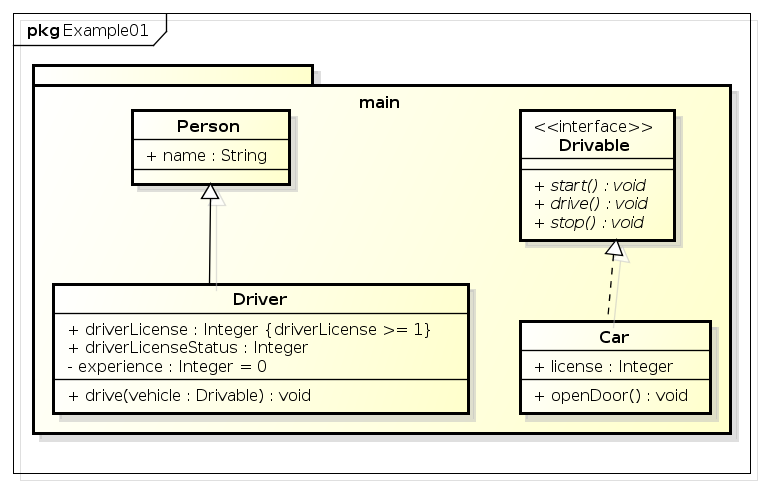
\includegraphics[width=.8\textwidth]{umlClassDiagramExample01_Diagram}
	\end{figure}
\end{frame}

\begin{frame}[t]
	\frametitle{UMLSequenceDiagram Concrete Syntax Example}
	\begin{figure}[H]
   		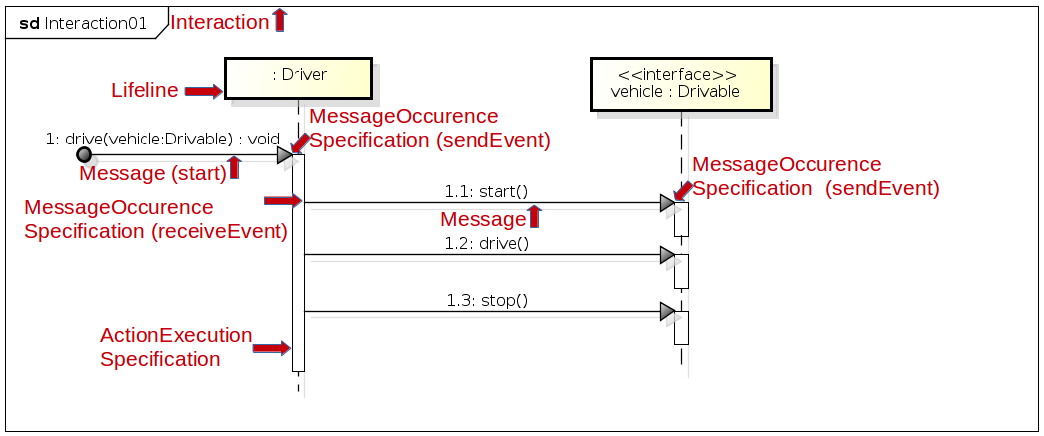
\includegraphics[width=\textwidth]{umlSequenceDiagramExample01_Diagram}
	\end{figure}
\end{frame}

\begin{frame}
	\frametitle{UMLContract}
	\begin{itemize}
		\item No concrete syntax defined
		\item Contraints (pre or postcondition or invariant) related to Properties or Operations
		\begin{itemize}
			\item Opaque Expression (textual definition)
			\item Interval
		\end{itemize}	
	\end{itemize}
\end{frame}

\begin{frame}
	\frametitle{Java Concrete Syntax Example}
	\nocite{heidenreich2009jamopp}
	\begin{figure}[H]
   		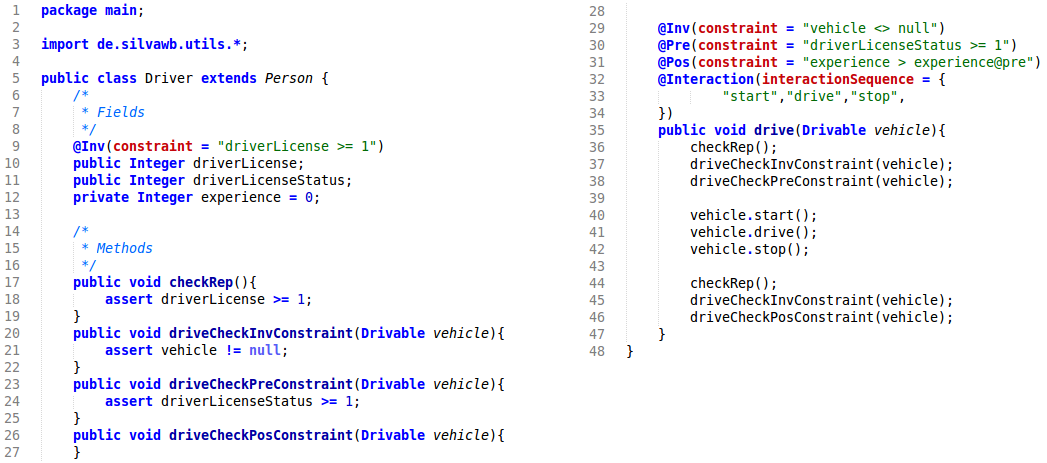
\includegraphics[width=\textwidth]{javaMetamodelExample01_Text}
	\end{figure}	
\end{frame}

%-------------------
% Subsection
%-------------------
\subsection{The Relations}
\begin{frame}
	\frametitle{The Relations}
	\tableofcontents[currentsection, currentsubsection] 
\end{frame}

\begin{frame}
	\frametitle{Triple Graphs}
	\nocite{hermann2011correctness}
	\begin{itemize}
		\item Relations coded by triple graphs
	\end{itemize}
	\begin{figure}
		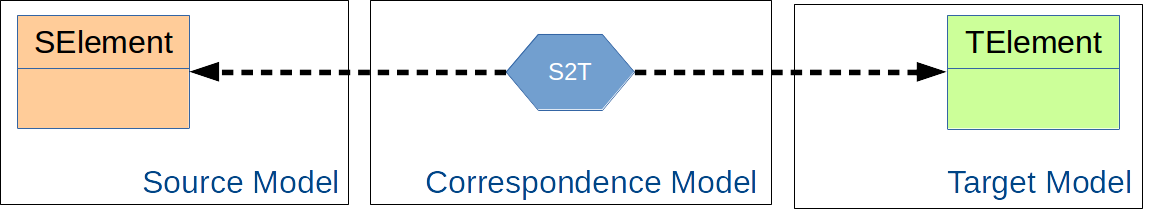
\includegraphics[width=.7\textwidth]{tripleGraphs}
	\end{figure}
	\pause
	\begin{itemize}
		\item Each edge of the network has a triple graphs grammar (TGG).
		\item A TGG is basically a grammar constructed upon triple graphs.
	\end{itemize}
\end{frame}

\begin{frame}
	\frametitle{UMLClassDiagram2java}
	\begin{figure}
		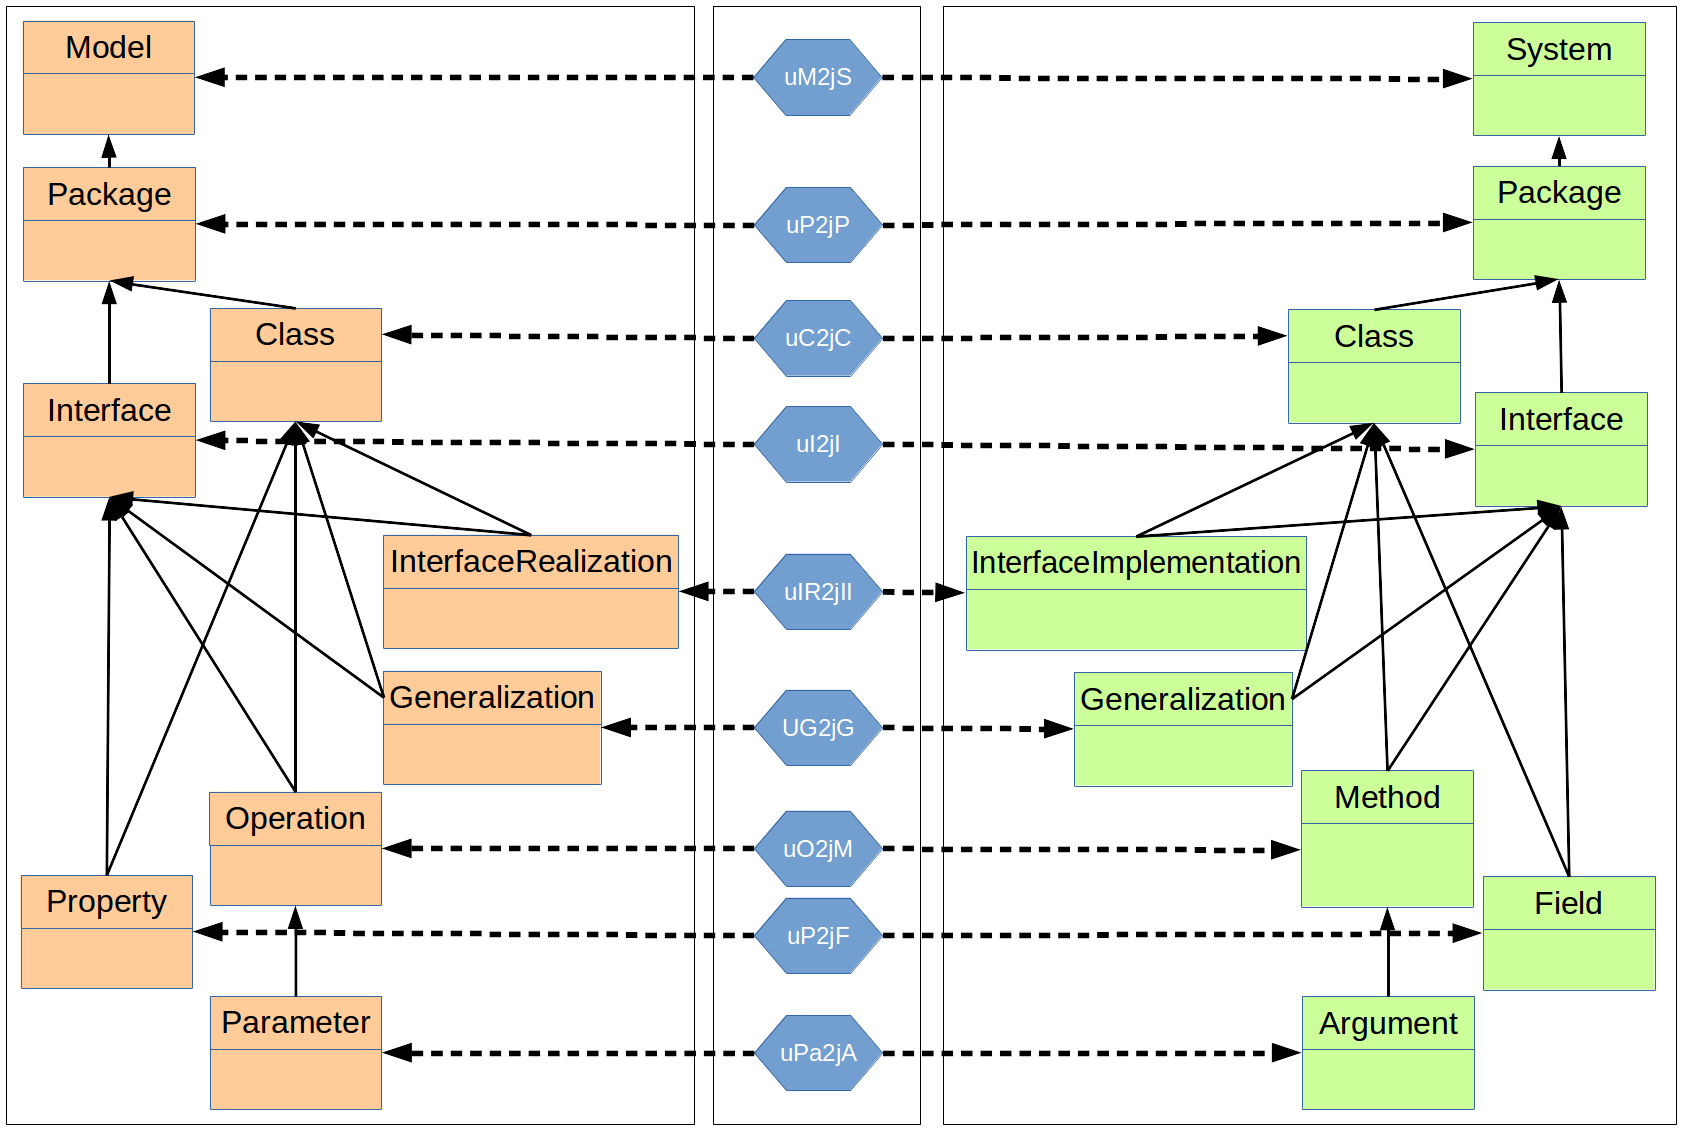
\includegraphics[width=.8\textwidth]{umlClassDiagram2java_type}
	\end{figure}
\end{frame}

\begin{frame}
	\frametitle{UMLSequenceDiagram2java}
	\begin{figure}
		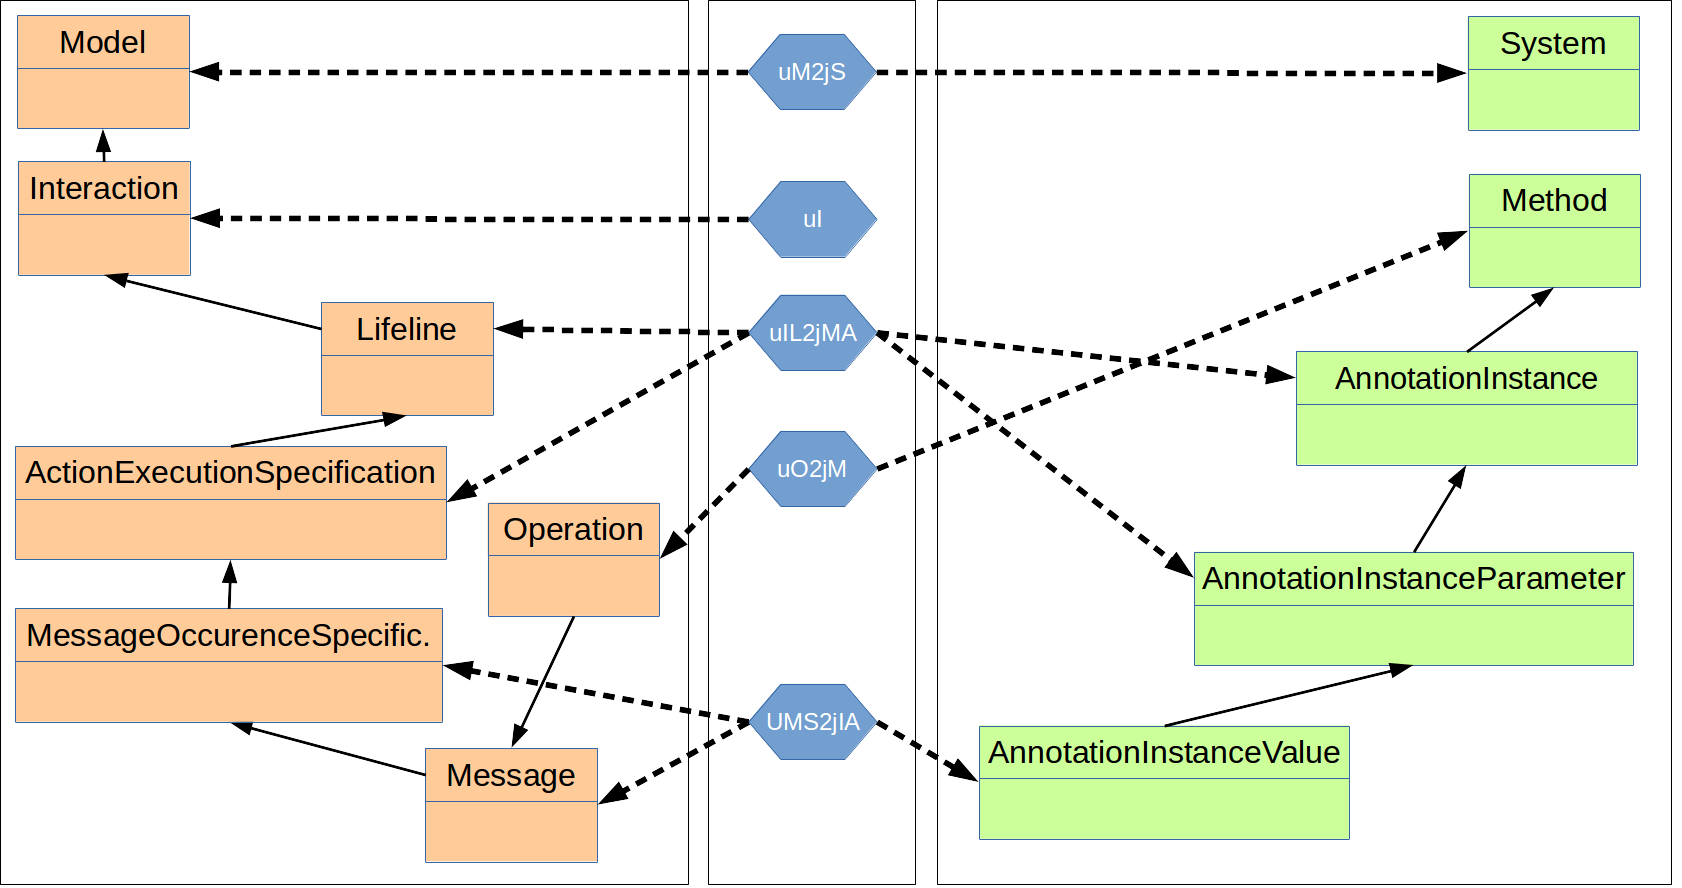
\includegraphics[width=.8\textwidth]{umlSequenceDiagram2java_type}
	\end{figure}
\end{frame}

\begin{frame}
	\frametitle{UMLContract2java}
	\begin{figure}
		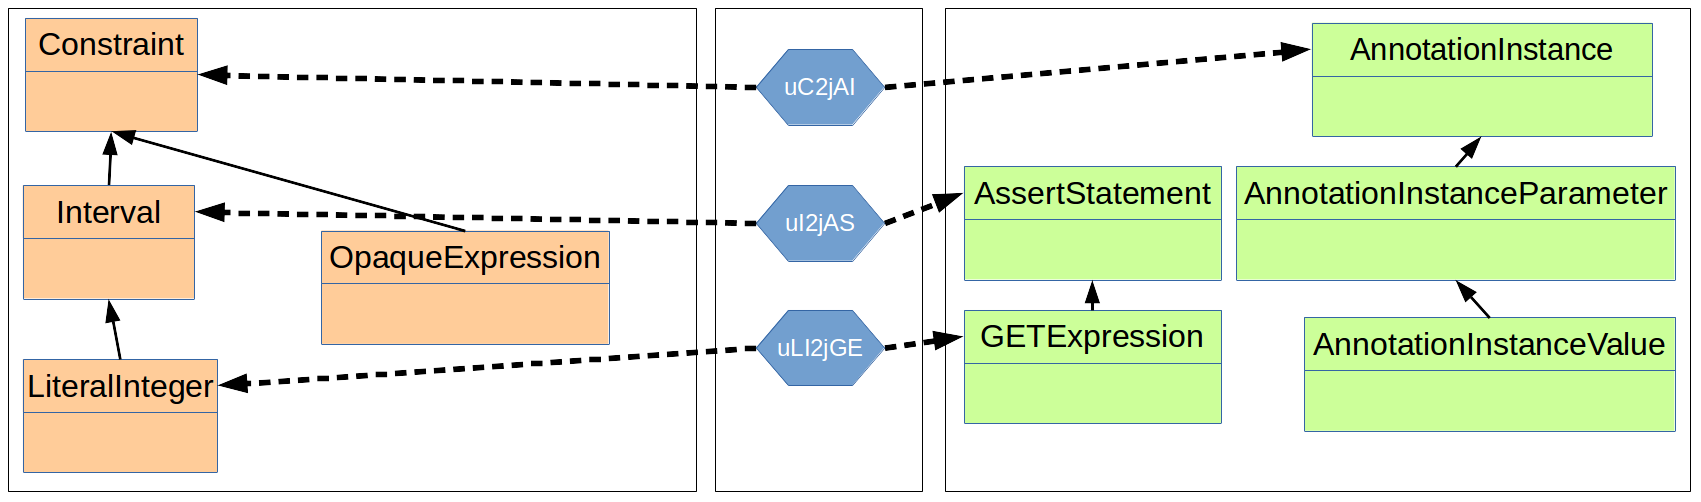
\includegraphics[width=.8\textwidth]{umlContract2java_type}
	\end{figure}
\end{frame}

%-------------------
% Subsection
%-------------------
\subsection{The Synchronization}
\begin{frame}
	\frametitle{The Synchronization}
	\tableofcontents[currentsection, currentsubsection] 
\end{frame}

\begin{frame}[t]
	\frametitle{Synchronization Scheme for Each TGG}
	\begin{itemize}
		\item Following scheme for every edge of the network of metamodels
	\end{itemize}
	\pause
	\begin{figure}
		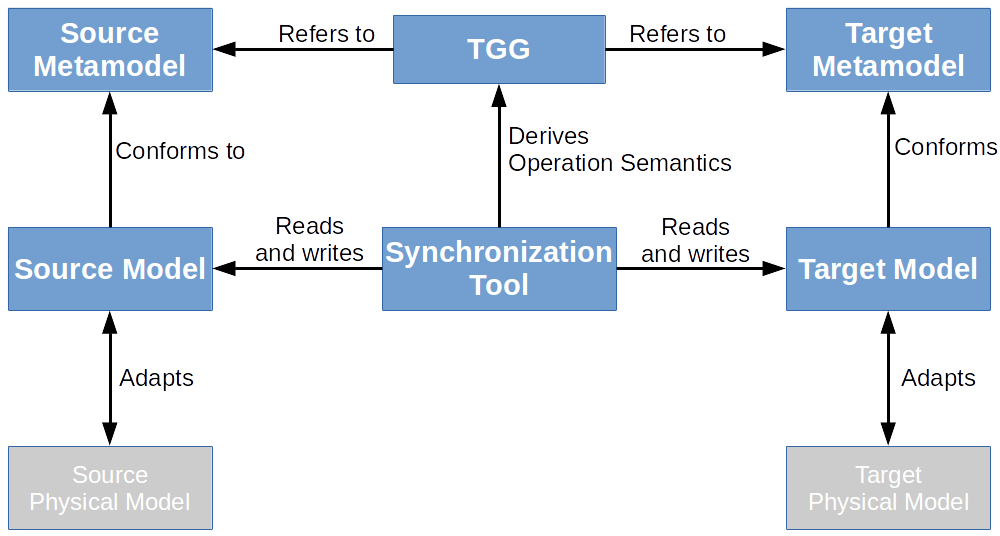
\includegraphics[width=.8\textwidth]{synchronization_scheme}
	\end{figure}
	\nocite{czarnecki2006feature}
	\nocite{giese2010model}
	\pause
	\begin{itemize}
		\item Treated separately by state-of-the-art approaches
		\pause
		\item How to treat the whole network of metamodels?
	\end{itemize}
\end{frame}

\begin{frame}[t]
	\frametitle{Synchronization Algorithm for the Network}
	{\footnotesize 
		\begin{algorithmic}
			\Function{Network Synchronization}{$G$, $v$, $v_{new}$, $\delta_v$}
				\State Update $v$ to $v_{new}$ in $G$
				\ForAll{$n_i = N(v)$}
								\State Synchronize $n_i$ according to $v$, $v_{new}$ and $\delta_v$
								\If{$n_i$ was modified}
									\State Network Synchronization (G, $n_i$, $n_{i_{new}}$, $\delta_n$)
								\EndIf
							\EndFor
				\State \Return G
			\EndFunction
		\end{algorithmic}
	}
	\pause
	\begin{itemize}
		\item Supposing only one modification at a time and unidirectional modifications.
		\item The algorithm always terminates (for $G$ finite without cycles).
		\item The algorithm is deterministic (for deterministic synchronization).
	\end{itemize}
\end{frame}


%------------------------------------------------
\section{Conclusion} % Sections can be created in order to organize your presentation into discrete blocks, all sections and subsections are automatically printed in the table of contents as an overview of the talk
%------------------------------------------------
\begin{frame}
	\frametitle{Conclusion}
	\tableofcontents[currentsection, currentsubsection] 
\end{frame}

\begin{frame}[t]
	\frametitle{Achieved goals}
	\begin{enumerate}
		\item Metamodel definitions of artifacts from the Java Technological Space
		\begin{itemize}
			\item Contributive for the use with TGG
			\item Simplifications and incompleteness
		\end{itemize}
		\pause
		\item Creation of a network of metamodels including the relations' formalizations
		\begin{itemize}
			\item Exploration of TGGs for defining the relations
			\item Evaluation of the definitions through forward transformation
			\item Simplifications
		\end{itemize}
		\pause
		\item The proposal of an algorithm for network synchronization
		\begin{itemize}
			\item Novel view of the model synchronization problem
			\item Assumptions
		\end{itemize}
	\end{enumerate}
\end{frame}

\begin{frame}
	\frametitle{Thank you}
	\begin{center}
		{\LARGE \textbf{Thank you for your attention}}
	\end{center}
\end{frame}

%------------------------------------------------
% Bibliography
%------------------------------------------------
\section{References}
%------------------------------------------------
\begin{frame}
	\frametitle{References}
	\tiny
	\bibliographystyle{plainnat}
	\bibliography{biblio}
\end{frame}
%------------------------------------------------

%------------------------------------------------
% Extra
%------------------------------------------------
\appendix

\begin{frame}
	\frametitle{Appendix}
	\begin{center}
		{\LARGE \textbf{Appendix}}
	\end{center}
\end{frame}

%%%%%%%%%%%%%%%%%%%%%% The Metamodels %%%%%%%%%%%%%%%%%%%%%%
\begin{frame}[t]
	\frametitle{UMLClassDiagram Abstract Syntax Example}
	\nocite{omg2007unified}
	\begin{figure}[H]
		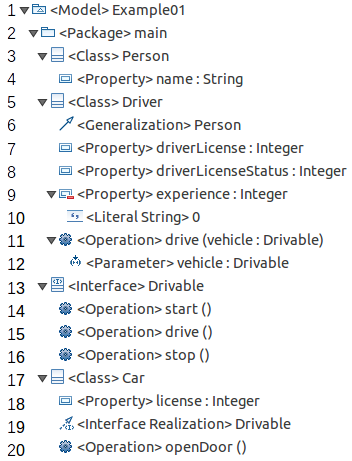
\includegraphics[width=.45\textwidth]{umlClassDiagramExample01}
	\end{figure}
\end{frame}

\begin{frame}[t]
	\frametitle{UMLClassDiagram Metamodel}
	\begin{figure}[H]
		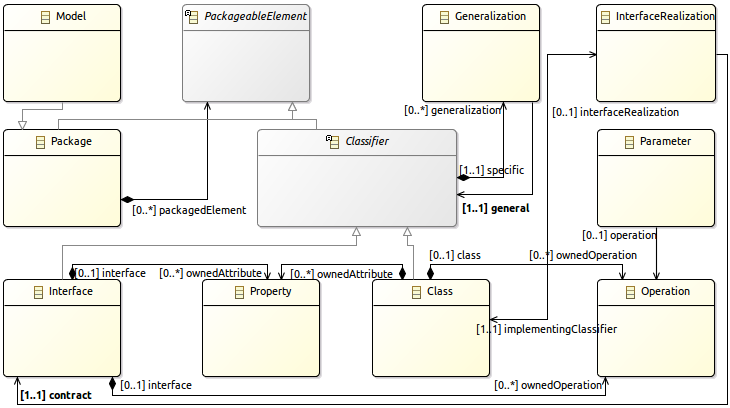
\includegraphics[width=\textwidth]{umlClassDiagramSimple01}
	\end{figure}
\end{frame}

\begin{frame}[t]
	\frametitle{UMLSequenceDiagram Abstract Syntax Example}
	\begin{figure}[H]
   		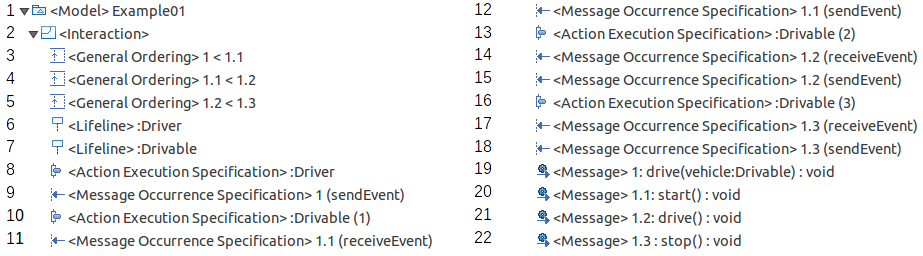
\includegraphics[width=\textwidth]{umlSequenceDiagramExample01}
	\end{figure}
\end{frame}

\begin{frame}[t]
	\frametitle{UMLSequenceDiagram Metamodel}
	\begin{figure}[H]
		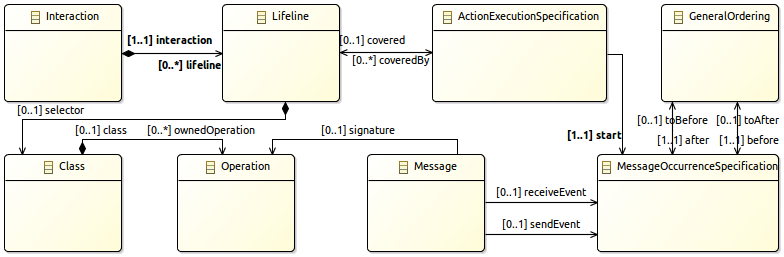
\includegraphics[width=\textwidth]{umlSequenceDiagramSimple01}
	\end{figure}
\end{frame}

\begin{frame}[t]
	\frametitle{UMLContract Abstract Syntax Example}
	\begin{figure}[H]
		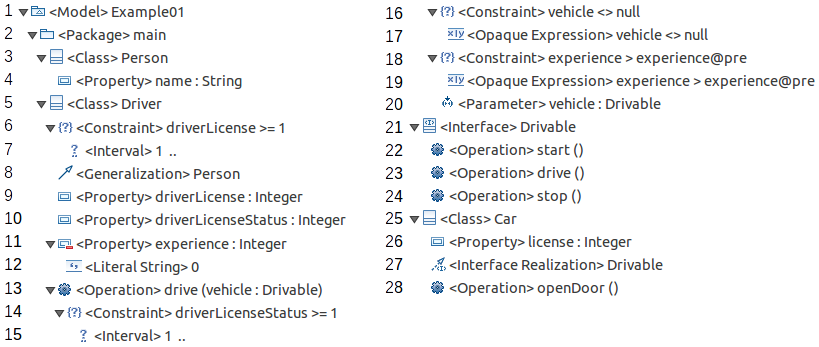
\includegraphics[width=\textwidth]{umlContractDiagramExample01}
	\end{figure}
\end{frame}

\begin{frame}[t]
	\frametitle{UMLContract Metamodel}
	\begin{figure}[H]
		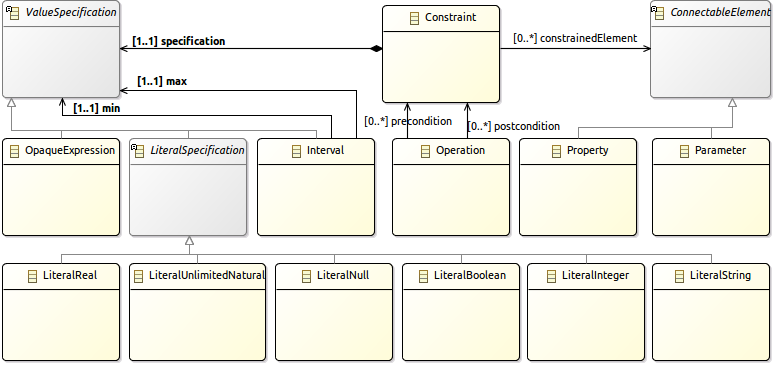
\includegraphics[width=\textwidth]{umlContractSimple01}
	\end{figure}
\end{frame}

\begin{frame}[t]
	\frametitle{Java Abstract Syntax Example}
	\vskip -10pt
	\begin{figure}[H]
		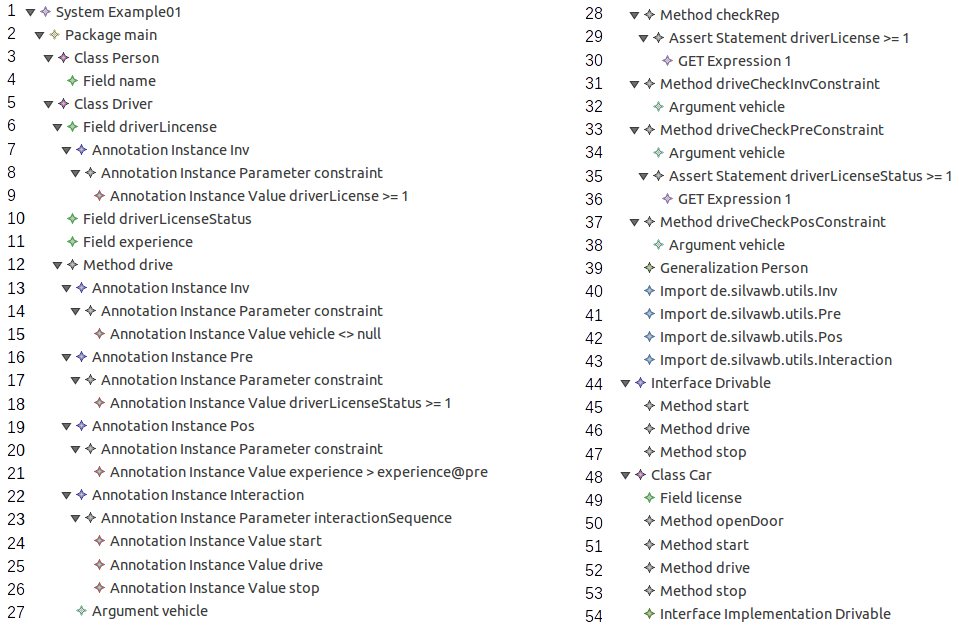
\includegraphics[width=\textwidth]{javaMetamodelExample01}
	\end{figure}
\end{frame}

\begin{frame}[t]
	\frametitle{Java Metamodel}
	\vskip -10pt
	\begin{figure}[H]
		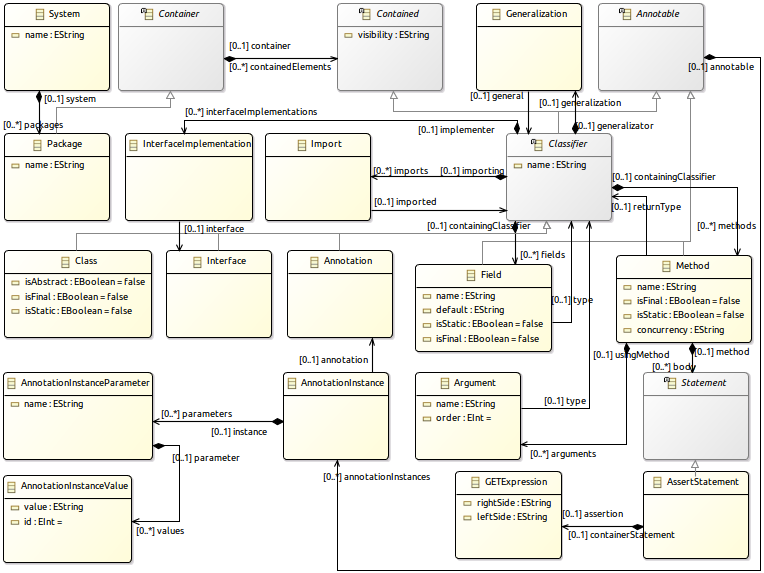
\includegraphics[width=.85\textwidth]{javaMetamodel}
	\end{figure}
\end{frame}

%%%%%%%%%%%%%%%%%%%%%% The Relations %%%%%%%%%%%%%%%%%%%%%%
\begin{frame}[t]
	\frametitle{Result of the implementation for UMLClassDiagram2java}
	\begin{itemize}
		\item Forward transformation was applied.
	\end{itemize}
	\begin{figure}
		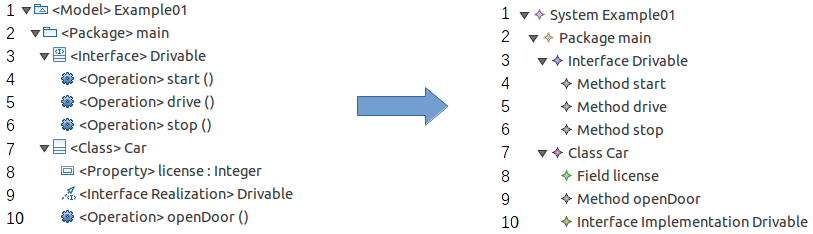
\includegraphics[width=\textwidth]{umlClassDiagram2java_Example01}
	\end{figure}
\end{frame}

\begin{frame}[t]
	\frametitle{Implementation for UMLSequenceDiagram2java}	
	\vskip -10pt
	\begin{itemize}
		\item Forward transformation was applied.
	\end{itemize}
	\begin{figure}
		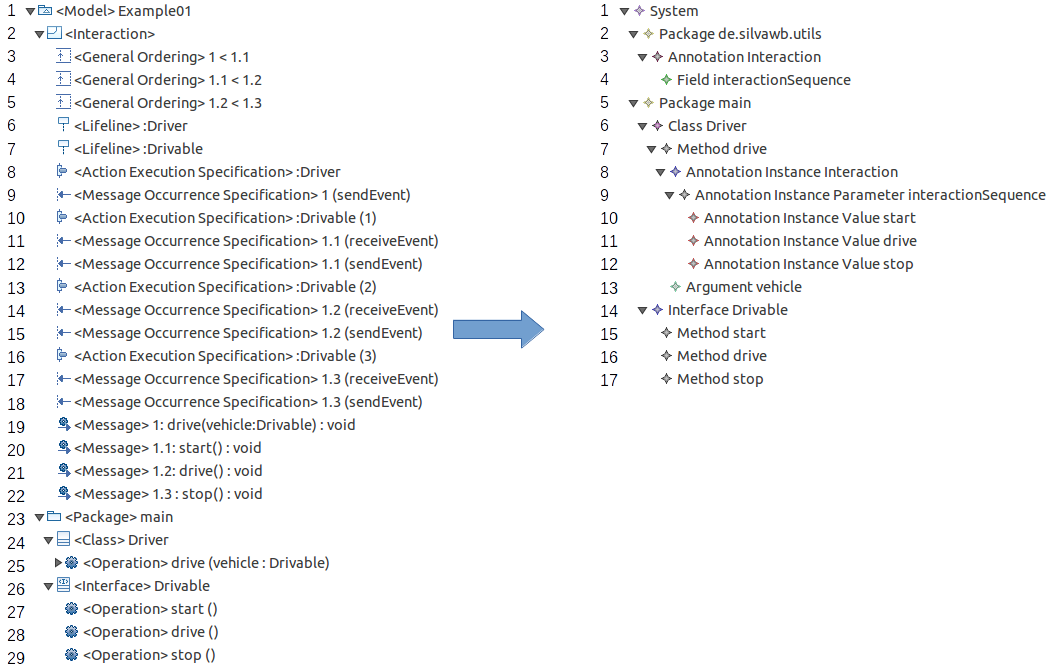
\includegraphics[width=.9\textwidth]{umlSequenceDiagram2java_Example01}
	\end{figure}
\end{frame}

\begin{frame}[t]
	\frametitle{Result of the Implementation for UMLContract2java}	
	\begin{itemize}
		\item Forward transformation was applied.
	\end{itemize}
	\begin{figure}
		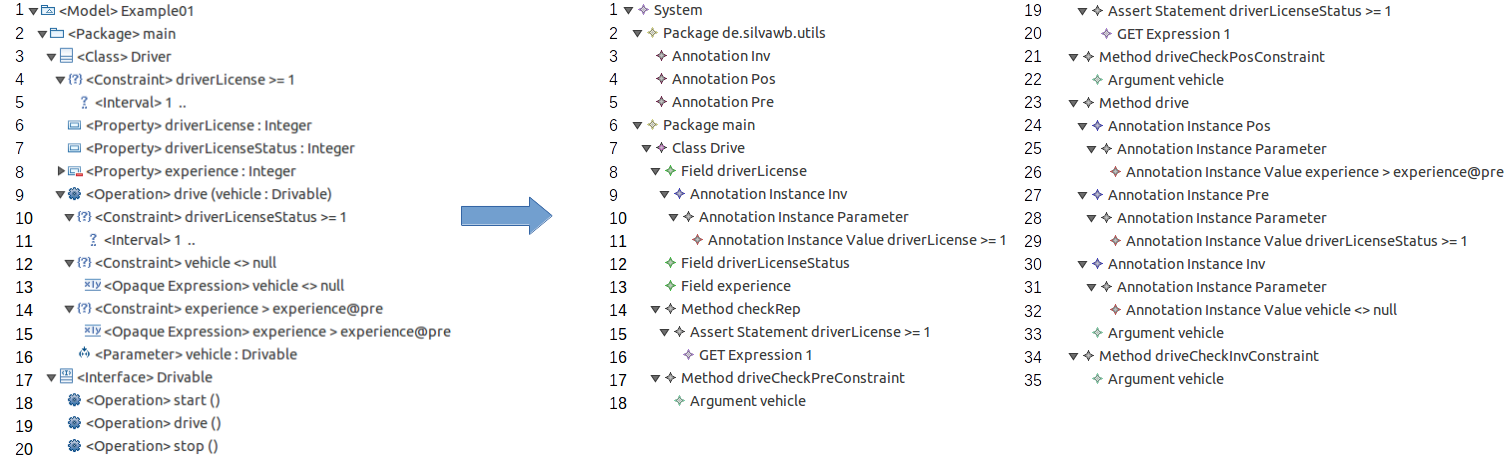
\includegraphics[width=\textwidth]{umlContracts2java_Example01}
	\end{figure}
\end{frame}
%----------------------------------------------------------------------------------------

\end{document}
